\documentclass[10pt,ignorenonframetext,,aspectratio=149]{beamer}
\usefonttheme{serif} % use mainfont rather than sansfont for slide text
\setbeamertemplate{caption}[numbered]
\setbeamertemplate{caption label separator}{: }
\setbeamercolor{caption name}{fg=normal text.fg}
\usepackage{lmodern}
\usepackage{amssymb,amsmath}
\usepackage{ifxetex,ifluatex}
\usepackage{fixltx2e} % provides \textsubscript
\ifnum 0\ifxetex 1\fi\ifluatex 1\fi=0 % if pdftex
  \usepackage[T1]{fontenc}
  \usepackage[utf8]{inputenc}
\else % if luatex or xelatex
  \ifxetex
    \usepackage{mathspec}
  \else
    \usepackage{fontspec}
  \fi
  \defaultfontfeatures{Ligatures=TeX,Scale=MatchLowercase}
  \newcommand{\euro}{€}
    \setmainfont[]{Open Sans}
\fi
% use upquote if available, for straight quotes in verbatim environments
\IfFileExists{upquote.sty}{\usepackage{upquote}}{}
% use microtype if available
\IfFileExists{microtype.sty}{%
\usepackage{microtype}
\UseMicrotypeSet[protrusion]{basicmath} % disable protrusion for tt fonts
}{}
\usepackage{graphicx,grffile}
\makeatletter
\def\maxwidth{\ifdim\Gin@nat@width>\linewidth\linewidth\else\Gin@nat@width\fi}
\def\maxheight{\ifdim\Gin@nat@height>\textheight0.8\textheight\else\Gin@nat@height\fi}
\makeatother
% Scale images if necessary, so that they will not overflow the page
% margins by default, and it is still possible to overwrite the defaults
% using explicit options in \includegraphics[width, height, ...]{}
\setkeys{Gin}{width=\maxwidth,height=\maxheight,keepaspectratio}

% Comment these out if you don't want a slide with just the
% part/section/subsection/subsubsection title:
\AtBeginPart{
  \let\insertpartnumber\relax
  \let\partname\relax
  \frame{\partpage}
}
\AtBeginSection{
  \let\insertsectionnumber\relax
  \let\sectionname\relax
  \frame{\sectionpage}
}
\AtBeginSubsection{
  \let\insertsubsectionnumber\relax
  \let\subsectionname\relax
  \frame{\subsectionpage}
}

\setlength{\emergencystretch}{3em}  % prevent overfull lines
\providecommand{\tightlist}{%
  \setlength{\itemsep}{0pt}\setlength{\parskip}{0pt}}
\setcounter{secnumdepth}{0}

\title{Estimating the Regression Model by Least Squares}
\author{Henrique Veras}
\date{}

%% Here's everything I added.
%%--------------------------

\usepackage{graphicx}
\usepackage{rotating}
%\setbeamertemplate{caption}[numbered]
\usepackage{hyperref}
\usepackage{caption}
\usepackage[normalem]{ulem}
%\mode<presentation>
\usepackage{wasysym}
%\usepackage{amsmath}


% Get rid of navigation symbols.
%-------------------------------
\setbeamertemplate{navigation symbols}{}

% Optional institute tags and titlegraphic.
% Do feel free to change the titlegraphic if you don't want it as a Markdown field.
%----------------------------------------------------------------------------------
\institute{PIMES/UFPE}

% \titlegraphic{\includegraphics[width=0.3\paperwidth]{\string~/Dropbox/teaching/clemson-academic.png}} % <-- if you want to know what this looks like without it as a Markdown field. 
% -----------------------------------------------------------------------------------------------------


% Some additional title page adjustments.
%----------------------------------------
\setbeamertemplate{title page}[empty]
%\date{}
\setbeamerfont{subtitle}{size=\small}

\setbeamercovered{transparent}

% Some optional colors. Change or add as you see fit.
%---------------------------------------------------
\definecolor{clemsonpurple}{HTML}{522D80}
 \definecolor{clemsonorange}{HTML}{F66733}
\definecolor{uiucblue}{HTML}{003C7D}
\definecolor{uiucorange}{HTML}{F47F24}


% Some optional color adjustments to Beamer. Change as you see fit.
%------------------------------------------------------------------
\setbeamercolor{frametitle}{fg=clemsonpurple,bg=white}
\setbeamercolor{title}{fg=clemsonpurple,bg=white}
\setbeamercolor{local structure}{fg=clemsonpurple}
\setbeamercolor{section in toc}{fg=clemsonpurple,bg=white}
% \setbeamercolor{subsection in toc}{fg=clemsonorange,bg=white}
\setbeamercolor{footline}{fg=clemsonpurple!50, bg=white}
\setbeamercolor{block title}{fg=clemsonorange,bg=white}


\let\Tiny=\tiny


% Sections and subsections should not get their own damn slide.
%--------------------------------------------------------------
\AtBeginPart{}
\AtBeginSection{}
\AtBeginSubsection{}
\AtBeginSubsubsection{}

% Suppress some of Markdown's weird default vertical spacing.
%------------------------------------------------------------
\setlength{\emergencystretch}{0em}  % prevent overfull lines
\setlength{\parskip}{0pt}


% Allow for those simple two-tone footlines I like. 
% Edit the colors as you see fit.
%--------------------------------------------------
\defbeamertemplate*{footline}{my footline}{%
    \ifnum\insertpagenumber=1
    \hbox{%
        \begin{beamercolorbox}[wd=\paperwidth,ht=.8ex,dp=1ex,center]{}%
      % empty environment to raise height
        \end{beamercolorbox}%
    }%
    \vskip0pt%
    \else%
        \Tiny{%
            \hfill%
		\vspace*{1pt}%
            \insertframenumber/\inserttotalframenumber \hspace*{0.1cm}%
            \newline%
            \color{clemsonpurple}{\rule{\paperwidth}{0.4mm}}\newline%
            \color{clemsonorange}{\rule{\paperwidth}{.4mm}}%
        }%
    \fi%
}

% Various cosmetic things, though I must confess I forget what exactly these do and why I included them.
%-------------------------------------------------------------------------------------------------------
\setbeamercolor{structure}{fg=blue}
\setbeamercolor{local structure}{parent=structure}
\setbeamercolor{item projected}{parent=item,use=item,fg=clemsonpurple,bg=white}
\setbeamercolor{enumerate item}{parent=item}

% Adjust some item elements. More cosmetic things.
%-------------------------------------------------
\setbeamertemplate{itemize item}{\color{clemsonpurple}$\bullet$}
\setbeamertemplate{itemize subitem}{\color{clemsonpurple}\scriptsize{$\bullet$}}
\setbeamertemplate{itemize/enumerate body end}{\vspace{.6\baselineskip}} % So I'm less inclined to use \medskip and \bigskip in Markdown.

% Automatically center images
% ---------------------------
% Note: this is for ![](image.png) images
% Use "fig.align = "center" for R chunks

\usepackage{etoolbox}

\AtBeginDocument{%
  \letcs\oig{@orig\string\includegraphics}%
  \renewcommand<>\includegraphics[2][]{%
    \only#3{%
      {\centering\oig[{#1}]{#2}\par}%
    }%
  }%
}

% I think I've moved to xelatex now. Here's some stuff for that.
% --------------------------------------------------------------
% I could customize/generalize this more but the truth is it works for my circumstances.

\ifxetex
\setbeamerfont{title}{family=\fontspec{Titillium Web}}
\setbeamerfont{frametitle}{family=\fontspec{Titillium Web}}
\usepackage[font=small,skip=0pt]{caption}
 \else
 \fi

% Okay, and begin the actual document...

\begin{document}
\frame{\titlepage}

\hypertarget{econometrics}{%
\section{Econometrics}\label{econometrics}}

\hypertarget{intro}{%
\subsection{Intro}\label{intro}}

\begin{frame}{Today}
\protect\hypertarget{today}{}
We now examine the Least Squares as an \textbf{estimator} of the
parameters of the linear regression model.

\vfill

We start by analysing the question ``\emph{why should we use least
squares}''?

\vfill

We will compare the LS estimator to other candidates based on their
\textbf{statistical properties}:

\begin{enumerate}
\tightlist
\item
  Unbiasedness
\item
  Efficiency
\item
  Consistency
\end{enumerate}

\vfill
\end{frame}

\hypertarget{population-orthogonality-conditions}{%
\subsection{Population orthogonality
conditions}\label{population-orthogonality-conditions}}

\begin{frame}{Population orthogonality}
\protect\hypertarget{population-orthogonality}{}
Recall assumption A3: \(E[\varepsilon_i|\mathbf{X}]=0\)

\vfill

By iterated expectations,
\(E[\varepsilon]= E_x {E[\varepsilon_i|\mathbf{X}]}=E_x[0]=0\).

\vfill

Also,
\(cov(\mathbf{x}, \mathbf{\varepsilon})=cov[\mathbf{x}, E[\varepsilon_i|\mathbf{X}]]=cov(\mathbf{x},0)=0\),
so \(\mathbf{x}\) and \(\mathbf{\varepsilon}\) are uncorrelated.

\vfill

From these results we can find that
\[E[\mathbf{Xy}]=E[\mathbf{X'X}]\mathbf{\beta}\]

\vfill
\end{frame}

\begin{frame}{Population orthogonality}
\protect\hypertarget{population-orthogonality-1}{}
Now recall the FOC of the LS problem: \(\mathbf{X'y}=\mathbf{X'Xb}\).
Dividing both sides by \(n\) and writing it as a summation:

\[\frac{1}{n}\sum_{i=1}^n{\mathbf{x_i y_i}}=\left(\frac{1}{n}\sum_{i=1}^n{\mathbf{x_i'x_i}}\right)\mathbf{b}\]

\vfill

Notice that this is the sample counterpart of the population condition
\(E[\mathbf{Xy}]=E[\mathbf{X'X}]\mathbf{\beta}\).
\end{frame}

\hypertarget{statistical-properties-of-the-ls-estimator}{%
\subsection{Statistical Properties of the LS
Estimator}\label{statistical-properties-of-the-ls-estimator}}

\begin{frame}{Statistical Properties of the LS Estimator}
\protect\hypertarget{statistical-properties-of-the-ls-estimator-1}{}
An \textbf{estimator} is a strategy for using the sample data that are
drawn from a population.

\vfill

The \textbf{properties} of that estimator are descriptions of how it can
be expected to behave when it is appied to a sample of data.
\end{frame}

\hypertarget{unbiasedness}{%
\subsection{Unbiasedness}\label{unbiasedness}}

\begin{frame}{Unbiasedness}
The least squares estimator is \textbf{unbiased} in every sample:

\vfill

\[E[\mathbf{b}|\mathbf{X}]=\mathbf{\beta}\]

Moreover,

\[E[\mathbf{b}]=E_x[E[\mathbf{b}|\mathbf{X}]]=E_x[\mathbf{\beta}]=\mathbf{\beta}\]

\vfill

This is to say that the Least Squares estimator has expectation
\(\mathbf{\beta}\).

\vfill

Moreover, when we average this over the possible values of
\(\mathbf{X}\), the unconditional mean is also \(\mathbf{\beta}\).

\vfill
\end{frame}

\begin{frame}{Omitted Variable Bias (OVB)}
\protect\hypertarget{omitted-variable-bias-ovb}{}
Suppose the true population model is given by
\[\mathbf{y}=\mathbf{X\beta}+\gamma z + \mathbf{\varepsilon}\]

\vfill

If we estimate \(\mathbf{y}\) on \(\mathbf{X}\) only, without the
\emph{relevant} variable \(z\), the estimator is

\[\begin{split}
\mathbf{b} & =(\mathbf{X}'\mathbf{X})^{-1}\mathbf{X}'\mathbf{y}=(\mathbf{X}'\mathbf{X})^{-1}\mathbf{X}'(\mathbf{X\beta}+\gamma z+\varepsilon) \\
 & = \mathbf{\beta}+(\mathbf{X}'\mathbf{X})^{-1}\mathbf{X}'\gamma z+(\mathbf{X}'\mathbf{X})^{-1}\mathbf{X}'\mathbf{\varepsilon}
 \end{split}\]

\vfill
\end{frame}

\begin{frame}{Omitted Variable Bias (OVB)}
\protect\hypertarget{omitted-variable-bias-ovb-1}{}
The expected value is given by

\[\begin{split}
E[\mathbf{b}|\mathbf{X},z] & =\mathbf{\beta}+(\mathbf{X}'\mathbf{X})^{-1}\mathbf{X}' \gamma z\\
 & = \mathbf{\beta} + \mathbf{p}_{X.z}\gamma,
\end{split}\]

where \(\mathbf{p}_{X.z}=(\mathbf{X}'\mathbf{X})^{-1}\mathbf{X}'z\).
What does it represent? What happens if \(\mathbf{X}\) and z are
orthogonal?

\vfill

Based on the FWL theorem and corollary 3.2.1, we can write

\[E[b_k|\mathbf{X},z]=\beta_k+\gamma\left(\frac{cov(z, x_k| \text{all other x's})}{var(x_k | \text{all other x's})}\right)\]

\vfill
\end{frame}

\begin{frame}{An Example}
\protect\hypertarget{an-example}{}
Suppose we are interested in estimating the returns to education
regression model below:

\[Income=\beta_0+\beta_1 Educ + \beta_2 age + \beta_3 age^2 + \beta_4 Abil + \varepsilon\]

\vfill

What is the sign of the bias if we estimate the model above without the
(\emph{unobserved}) \(Abil\)?

\vfill
\end{frame}

\begin{frame}{An Example}
\protect\hypertarget{an-example-1}{}
The sign of the bias will depend on the signs of \(\gamma\) and
\(cov(z, x_k| \text{all other x's})\):

\[E[b_1|\mathbf{X},z]=\beta_1+\gamma\left(\frac{cov(Abil, Educ | age, age^2)}{var(Educ | age, age^2)}\right)\]

\vfill

Thus, if \(\gamma>0\) and \(cov(Abil, Educ | age, age^2)>0\), \(b_1\)
will be biased upward: \[E[b_1|\mathbf{X},z]>\beta_1\]

\vfill

Notice, however, that in some circumstances, the sign of the conditional
covariance might not be obvious!

\vfill

What happens if we include irrelevant variables instead?
\end{frame}

\begin{frame}{Variance of the Least Squares Estimator}
\protect\hypertarget{variance-of-the-least-squares-estimator}{}
If Assumption A4 holds, the variance of the Least Squares estimator is
given by

\[Var(\mathbf{b}|\mathbf{X})=\sigma^2(\mathbf{X'X})^{-1}\]

\vfill

If we wish to find a sample estimate of \(Var(\mathbf{b}|\mathbf{X})\),
we need to estimate the (unknown) population parameter \(\sigma^2\).

\vfill

Recall:

\begin{enumerate}
\tightlist
\item
  \(\sigma^2\) is the variance of the error term:
  \(\sigma^2=E[\varepsilon_i^2|\mathbf{X}]\)
\item
  \(e_i\) is the estimate of \(\varepsilon_i\)
\end{enumerate}

\vfill
\end{frame}

\begin{frame}{Variance of the Least Squares Estimator}
\protect\hypertarget{variance-of-the-least-squares-estimator-1}{}
A natural estimator for \(\sigma^2\) would then be
\(\hat{\sigma}^2=\frac{1}{n} \sum_{i=1}^n{e_i^2}\).

\vfill

However, we would also need to estimate \(K\) parameters
\(\mathbf{\beta}\), which would distort \(\sigma^2\).

\vfill

An \textbf{unbiased} estimator for \(\sigma^2\) is
\[s^2=\frac{\mathbf{e}'\mathbf{e}}{n-K}\]

\vfill

Like \(\mathbf{b}\), \(s^2\) is unbiased unconditionally because
\[E[s^2]=E_X[E[s^2|\mathbf{X}]]=E_X[\sigma^2]=\sigma^2\]
\end{frame}

\begin{frame}{Variance of the Least Squares Estimator}
\protect\hypertarget{variance-of-the-least-squares-estimator-2}{}
The \textbf{standard error of the regression} is \(s=\sqrt{s^2}\).

\vfill

The variance of the Least Squares Estimator can thus be estimated by

\[\hat{Var}(\mathbf{b}|X)=s^2(\mathbf{X'X})^{-1}\]

\vfill

\(\hat{Var}(\mathbf{b}|X)\) is the sample estimate of the \emph{sampling
variance} of the LS estimator.

\vfill

Notice that the \(k\)-th diagonal element of this matrix is
\([s^2(\mathbf{X'X}_{kk})^{-1}]^{1/2}\), the standard error of the
estimator \(b_k\).
\end{frame}

\hypertarget{the-gauss-markov-theorem}{%
\subsection{The Gauss-Markov Theorem}\label{the-gauss-markov-theorem}}

\begin{frame}{The Gauss-Markov Theorem}
\protect\hypertarget{the-gauss-markov-theorem-1}{}
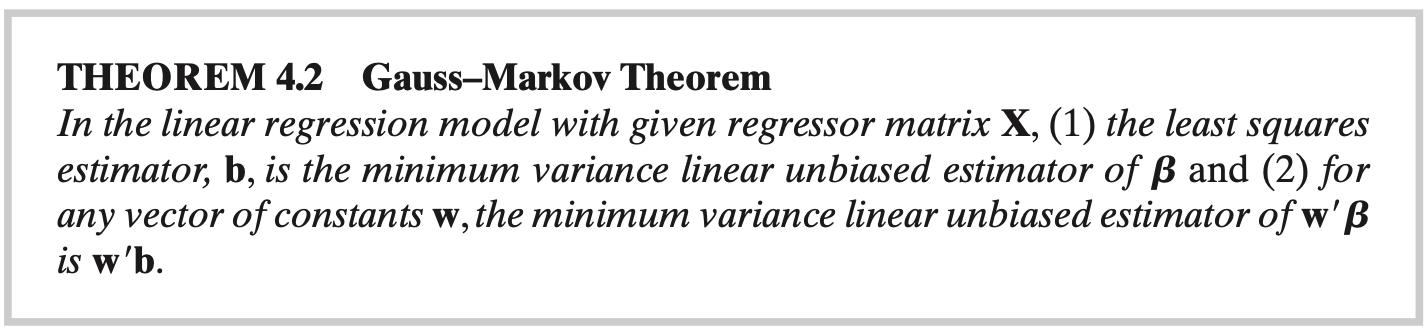
\includegraphics{/Users/henriquefonseca/Desktop/temp/Rmarkdown-practice/henriqueveras.github.io/files/Econometrics/Lecture Notes/3/theorem_4.2.png}
\end{frame}


\section[]{}
\frame{\small \frametitle{Table of Contents}
\tableofcontents}
\end{document}
